%% ------------------------------------------------------------------------- %%
\chapter{Hash Functions}
\label{cap:Hash Functions}

%% ------------------------------------------------------------------- %%
%\begin{itemize}
%\item Define Hash Function
%\item Give some examples of hash functions (Multiplicative / Remainder)
%\item Present Dragon Book metric and Evaluate hash functions
%\end{itemize}
%% ------------------------------------------------------------------- %%

Outside computer science, the word \textit{``hash''} in the english language means to ``chop'' or to ``mix'' something. This meaning is entirely related to what hash functions are supposed to do. hash functions are functions that are used to map data of an arbitrary size to data of a fized size \cite{HashFuncWiki}.

They have wide applications in computer science, being used in information and data scurity, compilers, distributed systems and hardcore algorithms. During this chapter I first define and explain the basics of a hash function, then I give an intiution in some metrics of what is a good hash function, as discussed in the famous \textit{``Red Dragon Book''} \cite{DragonBook} along with some reproduction of known results in the area.

The value extracted from the hash function for an object is usually called \textit{Hash Value}. The hash value is usually, but not necessarily, smaller than the object that generated it. For example, we can have a hash function that takes Gigabytes or Terabytes files and return an 8 bytes hash value.

\begin{figure}[h!]
  \centering
  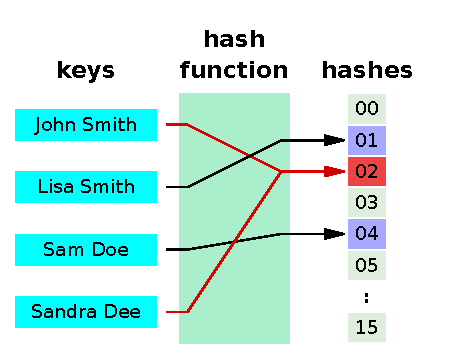
\includegraphics[width=10cm]{figuras/hash-function.pdf}
  \caption{Example of a hash function from string to 4 bit integer. }
\end{figure}

\bigskip

To formalize a little, lets define a hash function as a function \( H \) that takes an element \( x \in X \) and has \( [0, M) \) as a codomain.

\[ 0 \leq H(x) < M \]

\medskip

This is the same definition used by Donald Knuth \cite{TAOCP3} and some articles \cite{RobinHoodHashing}. This definition makes sense for our case because we will be talking mostly about hash functions used in hash tables, and in that case we want integers that will be indexes in an array (as we will se later on). In other cases will may see hash functions value as strings, like for when we hash an string for password storage or when we use a hash function in files for check-sum (for when we are checking if two files are the same). For the goal of this thesis we will not be focusing on those functions, but it is important to notice that strings can also be abstracted to integers if we just look at the bytes.

For our specific case we are looking at a hash function that is good for the construction of hash tables, that is that is fast to calculate and minimizes the number of collisions. Depending on our goals we might want a different metric, for check-sums for example we may want a function that is very sensible to chages, and for passwords one that is very hard to find its inverse.
